% =====================================================================
%  DeepREAP -- Springer LNNS (Lecture Notes in Networks and Systems)
%  Uses the standard Springer llncs document class (LNNS and LNCS share
%  the same class file).  Requires: llncs.cls, splncs04.bst (optional).
%  Compile with:  pdflatex deepreap  ->  pdflatex deepreap
% =====================================================================
\documentclass[runningheads]{llncs}

\usepackage{graphicx}
\usepackage{booktabs}
\usepackage{amsmath}
\usepackage{amssymb}
\usepackage{multirow}
\usepackage{url}
\usepackage[T1]{fontenc}

\graphicspath{{figures/}}

% Springer discourages \boldmath in tables; use \bfseries via booktabs.
\renewcommand{\arraystretch}{1.15}

\begin{document}

% ---------------------------------------------------------------------
\title{DeepREAP: Integrating a Regressive Ensemble Demand
Predictor with Deep Reinforcement Learning for Cloud Resource
Allocation}

\titlerunning{DeepREAP: Predictive Modeling Meets Deep RL Scheduling}

% TODO: confirm author list, affiliations and e-mail addresses before
% submission.  The names below are carried over from the original
% conceptual study; adjust to reflect the authorship of this
% implementation paper.
\author{%
Raghav Sharma\inst{1} \and
Rishabh Gupta\inst{1} \and
Suma Nagral\inst{1} \and
Shailaja Ramachandrapuram\inst{1}}

\authorrunning{R. Sharma et al.}

\institute{Department of Computer Engineering, San Jose State
University, San Jose, CA, USA\\
\email{\{raghav.sharma,rishabh.gupta,suma.nagral,shailaja.r\}@sjsu.edu}}

\maketitle
% ---------------------------------------------------------------------

\begin{abstract}
Cloud resource allocation is complicated by the dynamic and
heterogeneous nature of cloud workloads, and small and medium
enterprises (SMEs) disproportionately absorb the resulting
inefficiency. Prior work has advanced along two largely independent
axes: deep reinforcement learning (DRL) schedulers such as
DeepRM\_Plus, which react to the current cluster state, and regression
ensembles such as the Regressive Ensemble Approach for Prediction
(REAP), which forecast future demand. This paper presents DeepREAP, a
system coupling the two by injecting REAP's demand forecast directly
into the state representation of a convolutional DRL scheduler,
realizing as working software an architecture previously described
only conceptually. On a 60-day synthetic trace the REAP ensemble
attains an MSE of 8.07 on the CPU-load target, improving on every
constituent regressor. On a shared 3\,000-job trace the DeepREAP
imitation policy reduces average job slowdown to 8.27, against 20.11
for shortest-job-first and 18.76 for a Tetris-style packer --- a
2.4$\times$ improvement --- and lowers average completion time from
49.51 to 19.04 slots. We report these gains alongside their costs: the
policy completes fewer jobs within a fixed step budget, and our PPO
refinement stage degrades rather than improves the imitation
checkpoint at the training budget available. All code, seeds and
figures are released to support replication.

\keywords{Cloud resource allocation \and Deep reinforcement learning
\and Ensemble regression \and Job scheduling \and Demand prediction
\and Imitation learning.}
\end{abstract}

% =====================================================================
\section{Introduction}
% =====================================================================

Cloud computing has reshaped how organizations store and process data,
and at the centre of that shift sits resource allocation: the problem
of distributing compute, memory and network capacity across the
applications running on a platform. Allocation quality determines
service performance, operating cost and, ultimately, user experience.
It is also hard, because cloud environments are dynamic and the
demands placed on them are heterogeneous.

Small and medium enterprises (SMEs) feel this acutely. They rarely
employ dedicated capacity-planning staff, and they lack the scale over
which large providers amortize over-provisioning. An allocation policy
that is merely adequate at hyperscale can be materially expensive for
an SME.

Two families of machine-learning techniques have been brought to bear.
Deep reinforcement learning (DRL) schedulers learn an allocation
policy directly from interaction with the cluster; DeepRM~\cite{mao2016}
and its successor DeepRM\_Plus~\cite{guo2021} are the canonical
examples. Separately, regression models forecast future resource
demand from historical telemetry, enabling provisioning decisions to be
made before demand materializes~\cite{bankole2013,kaur2019}. The two
approaches are complementary --- one is reactive and optimizes
sequencing, the other is anticipatory --- yet they are seldom combined.

An earlier conceptual study by the present authors proposed DeepREAP,
an architecture uniting the REAP ensemble predictor~\cite{kaur2019}
with the DeepRM\_Plus scheduler~\cite{guo2021}. That study was
explicitly limited to a plan and a theoretical framework; it conducted
no implementation, testing or validation, and stated that the
system's real-world viability remained speculative. The present paper
closes that gap.

We contribute a working DeepREAP implementation --- REAP prediction,
DRL scheduling, an integration protocol and a monitoring loop as
runnable software rather than a specification; a concrete state-fusion
mechanism that injects a demand forecast into the scheduler's state as
additional image channels, requiring no change to the policy
architecture and no hand-coded contract between predictor and agent;
and an empirical evaluation against heuristic and DRL baselines on a
shared trace. We report the negative results alongside the positive
ones: PPO refinement does not improve on the imitation checkpoint at
the budget we could afford, and the ensemble does not dominate its
base models on every target.

Three questions guide the study. \textbf{RQ1:} how can regression
models be integrated into DeepRM\_Plus to improve demand prediction?
\textbf{RQ2:} what impact does that integration have on job completion
time and scheduling performance? \textbf{RQ3:} to what extent can it
reduce operational costs for SMEs?

% =====================================================================
\section{Related Work}
% =====================================================================

\textbf{Learning to schedule.} Early approaches allocate by priority:
Son and Buyya~\cite{son2019} combine priority-aware VM allocation with
bandwidth provisioning in SDN-enabled clouds, and Savitha and
Salvi~\cite{savitha2021} learn application priorities from historical
usage. Reinforcement learning removes the need for hand-designed
priority rules. Mao et al.~\cite{mao2016} introduced DeepRM,
formulating cluster scheduling over an image-like state encoding and
outperforming classical heuristics; Guo et al.~\cite{guo2021} extended
it into DeepRM\_Plus, using imitation learning to accelerate
convergence and improving average weighted turnaround time; Zhou
et al.~\cite{zhou2021} pair a DRL agent with a policy set enforcing
SLA constraints. Recurring concerns across this line of work are
generalizability, scalability, and the data appetite of training.

\textbf{Learning to predict.} A parallel literature forecasts demand
rather than sequencing it. Bankole and Ajila~\cite{bankole2013} find
SVM strongest among classical regressors for provisioning prediction
(4.5\,\% average error), Osypanka and
Nawrocki~\cite{osypanka2022,osypanka2023} report up to 85\,\% cost
reduction from ARIMA-based and self-adapting predictors, and Gyeera
et al.~\cite{gyeera2023} reach $R^2 = 0.9991$ with Boosted Decision
Trees at appreciable training cost. Most relevant here, Kaur, Bala and
Chana~\cite{kaur2019} propose REAP, which selects features by genetic
algorithm, trains multiple regressors on the selected subset, and
combines them in an accuracy-weighted ensemble, reaching 95\,\%
accuracy on a real-world dataset.

\textbf{The gap.} DRL schedules well; regression ensembles predict
well. Their integration into a single framework --- in which
anticipated demand conditions the scheduling policy itself --- remains
underexplored, and is the subject of this paper.

% =====================================================================
\section{System Design and Implementation}
% =====================================================================

DeepREAP chains four stages. A workload generator produces resource
telemetry and a job trace. REAP consumes the telemetry and forecasts
per-resource demand. The forecast is fused into the state
representation of a DeepRM\_Plus-style CNN scheduler, which emits
allocation decisions. A REST service exposes prediction and scheduling
endpoints, and Prometheus/Grafana close a monitoring loop in which
observed values submitted to a feedback endpoint update a
prediction-error gauge. The critical design choice is that forecasts
are \emph{fused into the state} rather than post-processed into a
priority score, so the policy learns for itself how much to trust
them.

\subsection{Workload Generation}

The original proposal assumed the availability of historical resource
usage without specifying a trace. We generate one with realistic
structure.

\textbf{Resource usage.} Hourly records for four service types (Web,
Database, Media, Compute) with diurnal and weekly cycles, an
autoregressive dependence on the previous hour's CPU, and Gaussian
noise. Default: 60 days $\times$ 4 services $=$ 5\,760 rows.

\textbf{Job trace.} Poisson arrivals; bimodal durations (80\,\% short
jobs of 1--3 slots, 20\,\% long jobs of 10--15 slots); bimodal
per-resource demand with one dominant resource per job, matching the
regime used by Mao et al.~\cite{mao2016}. Default: 3\,000 jobs over
1\,500 timesteps.

\subsection{REAP}

\textbf{Feature selection.} A chromosome is a binary mask over
candidate features. Fitness is
$-\mathrm{CV\_MSE} - 0.01 \cdot |\text{features}|$
for a Ridge regressor on the selected subset, with 3-fold
cross-validation, 25 generations, population 24, tournament-3
selection, single-point crossover and 5\,\% mutation.

\textbf{Base regressors.} Linear Regression, Bayesian Ridge, Decision
Tree, Random Forest and SVR with an RBF kernel --- the model families
named in the REAP formulation~\cite{kaur2019}.

\textbf{Ensemble.} Each model $m$ receives weight
$w_m \propto 1/\mathrm{MSE}_m$ on a held-out validation split,
normalized so that $\sum_m w_m = 1$.

\subsection{Scheduling Environment}

A discrete-time cluster scheduler with 2 resources of capacity 10 and
time horizon $T = 20$; $M = 5$ visible job slots plus a bounded
backlog of 60. The state image is
$[\text{cluster load} \mid \text{job}_1 \mid \dots \mid \text{job}_M]$
with shape $(1, R, T \cdot (M{+}1))$. Successful schedules do not
advance time, allowing the agent to fill several slots per timestep.
The reward at each time-advancing step is
$-\sum_j 1/T_j$ over resident jobs, scaled by $1/10$ to keep the PPO
value loss numerically stable.

\subsection{Forecast Fusion}

Given a forecast request, REAP is rolled forward $T$ hours to produce
a tensor of shape $(C, R, T)$ appended to the state image as extra
channels: channel 0 carries predicted CPU demand broadcast across the
resource axis and normalized to $[0,1]$; channel 1 carries predicted
memory demand under the same convention. The agent has no hard-coded
contract with these channels --- it learns during training whether and
how to weigh them. This is the mechanism by which DeepREAP differs
from vanilla DeepRM\_Plus, and it is the only difference between the
two configurations we compare.

\subsection{Policy Network and Training}

The policy is two \texttt{Conv2d} blocks with $(1,3)$ kernels, an
\texttt{AdaptiveAvgPool2d} to $(1,16)$, and an MLP head emitting
action logits and a value estimate. The adaptive pool makes the head
size independent of $T \cdot (M{+}1)$, which simplifies configuration
sweeps.

\textbf{Imitation pre-training.} An SJF expert is run for 30 episodes,
yielding roughly 6\,000 $(\text{state}, \text{action})$ pairs on which
the CNN is trained by cross-entropy for 6 epochs. Loss reaches 0.53 on
a 6-class problem, against a uniform-prior loss of $\ln 6 \approx
1.79$.

\textbf{PPO refinement.} Clipped-objective PPO with GAE
($\gamma = 0.995$, $\lambda = 0.95$, clip $= 0.1$, lr $= 1\text{e-}4$,
4 environments $\times$ 256-step rollouts, 3 epochs per update,
$c_{vf} = 0.25$, $c_{ent} = 0.01$, gradient-norm clip 0.5), run for 15
updates. Both the imitation and post-PPO checkpoints are saved and
benchmarked separately.

\subsection{Service and Monitoring Layer}

A FastAPI service exposes \texttt{/health}, \texttt{/predict},
\texttt{/forecast}, \texttt{/schedule}, \texttt{/feedback} and
\texttt{/metrics}. Models load from a configurable directory at
startup; a missing model yields HTTP 503 on the affected endpoint
rather than a crash. Prometheus scrapes \texttt{/metrics} every 5\,s
and Grafana is provisioned with a dashboard covering request rate,
latency percentiles, latest predicted value per target, observed
absolute error, and scheduling-decision rate.

% =====================================================================
\section{Experimental Setup}
% =====================================================================

All schedulers are evaluated on the \emph{same} job trace (seed 123)
for a budget of 201 environment steps. Seeds are fixed throughout ---
data generation 42/43, REAP 42, DeepRM 42, benchmark 123 --- so runs
are reproducible on identical hardware. We report:

\begin{itemize}
\item \textbf{Average slowdown} --- job turnaround normalized by
job duration (lower is better);
\item \textbf{Average completion time} --- in time slots
(lower is better);
\item \textbf{Jobs completed} ($n_{\text{done}}$) within the step
budget (higher is better);
\item \textbf{Total reward} --- the environment objective.
\end{itemize}

We compare seven schedulers: three heuristics (FIFO, SJF, Packer ---
a Tetris-style policy selecting the visible job whose demand vector
maximizes the dot product with free capacity), and the imitation and
post-PPO checkpoints of both DeepRM\_Plus and DeepREAP.

% =====================================================================
\section{Results}
% =====================================================================

\subsection{Prediction Accuracy (RQ1)}

Table~\ref{tab:reap-cpu} reports per-model error on the CPU-load
target. The ensemble improves on every constituent regressor on both
MSE and MAE, confirming that accuracy-weighted combination is
worthwhile for this target. The genetic algorithm selected 8 of 11
candidate features, discarding \texttt{day\_of\_week},
\texttt{is\_weekend} and \texttt{svc\_Database} --- information
already carried by \texttt{hour\_of\_day}, the autoregressive term and
the remaining one-hot indicators.

\begin{table}[t]
\centering
\caption{REAP base-model and ensemble accuracy on the
\texttt{cpu\_load} target (60-day trace). The ensemble improves on
every base model.}
\label{tab:reap-cpu}
\begin{tabular}{lrrr}
\toprule
\textbf{Model} & \textbf{MSE} & \textbf{MAE} &
\textbf{Ensemble weight} \\
\midrule
Linear Regression & 9.33  & 2.45 & 0.205 \\
Bayesian Ridge    & 9.34  & 2.45 & 0.205 \\
Decision Tree     & 14.47 & 2.99 & 0.132 \\
Random Forest     & 8.41  & 2.32 & 0.227 \\
SVR (RBF)         & 8.26  & 2.30 & 0.231 \\
\midrule
\textbf{Ensemble} & \textbf{8.07} & \textbf{2.28} & --- \\
\bottomrule
\end{tabular}
\end{table}

The picture on the memory-usage target is different, and we report it
plainly. As Table~\ref{tab:reap-mem} shows, the ensemble (MSE 25.04)
does \emph{not} improve on its strongest constituent, SVR (MSE 24.49).
Inverse-MSE weighting assigns SVR only 0.227 of the total weight, so
the ensemble is dragged toward the weaker linear and tree models. The
ensemble still beats four of five base models and remains a reasonable
default when the best base model is not known in advance, but the
claim that ensembling dominates unconditionally is not supported by
our data. A weighting scheme with sharper concentration --- softmax
over $-\mathrm{MSE}$ with a temperature parameter, or simple top-$k$
selection --- would likely recover the gap.

\begin{table}[t]
\centering
\caption{REAP accuracy on the \texttt{memory\_usage} target. Here SVR
alone outperforms the ensemble; see the discussion in
Sect.~\ref{sec:results}.}
\label{tab:reap-mem}
\begin{tabular}{lrrr}
\toprule
\textbf{Model} & \textbf{MSE} & \textbf{MAE} &
\textbf{Ensemble weight} \\
\midrule
Linear Regression & 27.50 & 4.23 & 0.202 \\
Bayesian Ridge    & 27.50 & 4.23 & 0.202 \\
Decision Tree     & 34.68 & 4.69 & 0.160 \\
Random Forest     & 26.47 & 4.13 & 0.210 \\
\textbf{SVR (RBF)} & \textbf{24.49} & \textbf{4.00} & 0.227 \\
\midrule
Ensemble          & 25.04 & 4.03 & --- \\
\bottomrule
\end{tabular}
\end{table}

\begin{figure}[t]
\centering
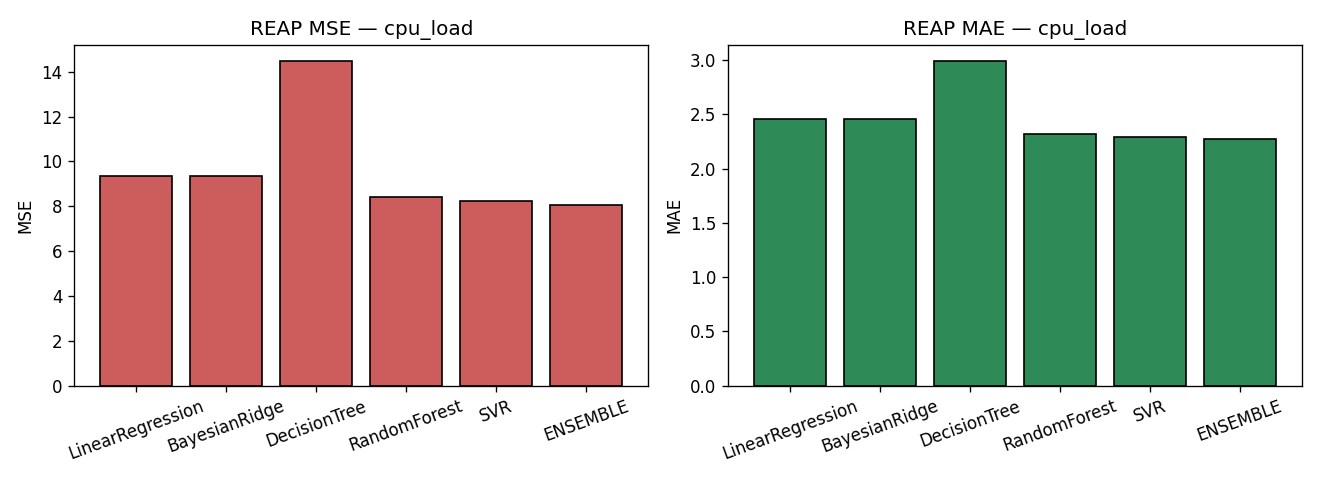
\includegraphics[width=0.88\textwidth]{reap_quality_cpu_load.png}
\caption{REAP base-model and ensemble error on the \texttt{cpu\_load}
target. Left: mean squared error. Right: mean absolute error. The
ensemble bar is lowest in both panels.}
\label{fig:reap-quality-cpu}
\end{figure}

\begin{figure}[t]
\centering
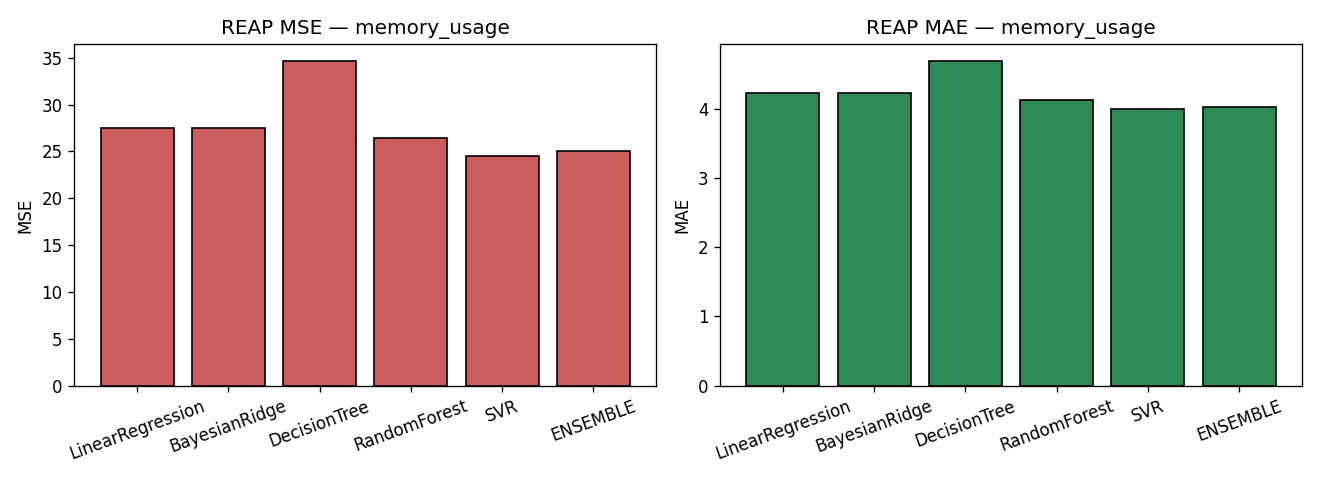
\includegraphics[width=0.88\textwidth]{reap_quality_memory_usage.png}
\caption{REAP error on the \texttt{memory\_usage} target. In contrast
to Fig.~\ref{fig:reap-quality-cpu}, the SVR bar edges below the
ensemble, illustrating the limits of inverse-MSE weighting when one
base model is clearly strongest.}
\label{fig:reap-quality-mem}
\end{figure}

\begin{figure}[t]
\centering
\begin{minipage}{0.49\textwidth}
\centering

\includegraphics[width=\textwidth]{reap_weights_cpu_load.png}
\end{minipage}
\hfill
\begin{minipage}{0.49\textwidth}
\centering
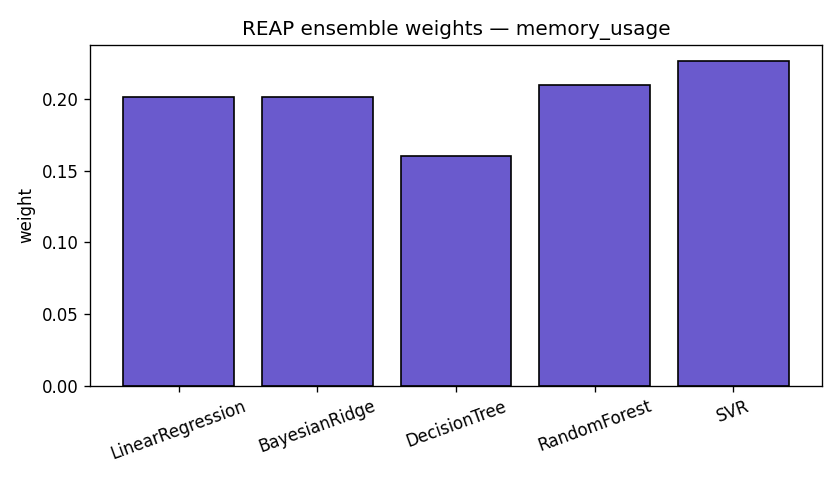
\includegraphics[width=\textwidth]{reap_weights_memory_usage.png}
\end{minipage}
\caption{Accuracy-derived ensemble weights for the \texttt{cpu\_load}
(left) and \texttt{memory\_usage} (right) targets. Weights are
narrowly spread --- from 0.13 to 0.23 --- because inverse-MSE
weighting is close to uniform when base-model errors are of similar
magnitude.}
\label{fig:reap-weights}
\end{figure}

Figure~\ref{fig:reap-weights} makes the weighting behaviour explicit:
across both targets the weights span only 0.13--0.23. The Decision
Tree, with roughly $1.7\times$ the MSE of SVR, is penalized far less
than that ratio would suggest. This near-uniformity is the direct
cause of the memory-target result above.

\subsection{Scheduling Performance (RQ2)}
\label{sec:results}

Table~\ref{tab:bench} and Figs.~\ref{fig:slowdown}--\ref{fig:completion}
report the scheduling benchmark.

\begin{table}[t]
\centering
\caption{Scheduler comparison on a shared job trace (seed 123, 201
steps). Arrows indicate the preferred direction. DeepREAP's imitation
policy attains the best slowdown and completion time; it also
completes the fewest jobs.}
\label{tab:bench}
\begin{tabular}{lrrrr}
\toprule
\textbf{Scheduler} & \textbf{Slowdown} $\downarrow$ &
\textbf{Completion} $\downarrow$ & \textbf{$n_{\text{done}}$}
$\uparrow$ & \textbf{Reward} \\
\midrule
FIFO                    & 20.20 & 48.65 & 54 & $-374.6$ \\
SJF                     & 20.11 & 49.51 & 53 & $-366.3$ \\
Packer                  & 18.76 & 48.42 & 52 & $-375.3$ \\
\midrule
DeepRM\_Plus (imitation) & 19.30 & 43.41 & 41 & $-414.1$ \\
DeepRM\_Plus (PPO)       & 24.47 & 55.44 & 41 & $-443.7$ \\
\midrule
\textbf{DeepREAP (imitation)} & \textbf{8.27} & \textbf{19.04} & 25 &
$-446.4$ \\
DeepREAP (PPO)          & 18.12 & 42.05 & 43 & $-401.8$ \\
\bottomrule
\end{tabular}
\end{table}

\begin{figure}[t]
\centering
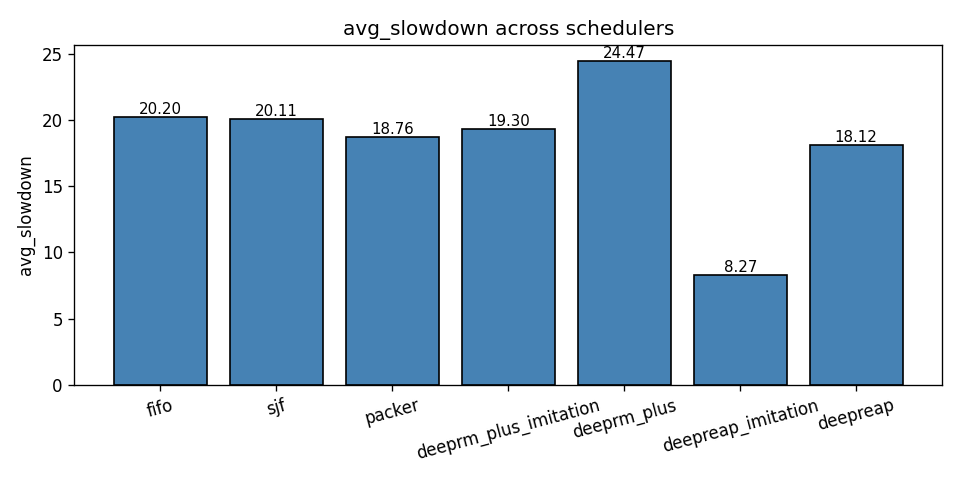
\includegraphics[width=0.78\textwidth]{avg_slowdown.png}
\caption{Average job slowdown across all seven schedulers (lower is
better). DeepREAP's imitation policy reaches 8.27, less than half the
best heuristic result of 18.76.}
\label{fig:slowdown}
\end{figure}

\begin{figure}[t]
\centering
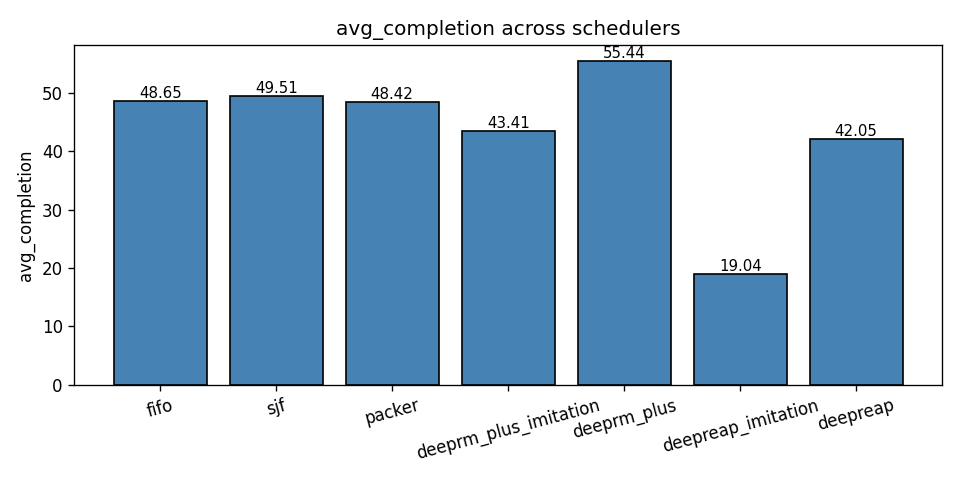
\includegraphics[width=0.78\textwidth]{avg_completion.png}
\caption{Average job completion time in slots (lower is better). The
ordering closely tracks Fig.~\ref{fig:slowdown}.}
\label{fig:completion}
\end{figure}

\textbf{The headline result.} DeepREAP's imitation policy achieves an
average slowdown of 8.27 against 20.11 for SJF and 18.76 for the
Packer heuristic --- a $2.4\times$ improvement over the best baseline
--- and cuts average completion time from 48.4--49.5 slots to 19.04.
Comparing DeepREAP against DeepRM\_Plus under identical training and
evaluation conditions isolates the contribution of the forecast
channels: slowdown falls from 19.30 to 8.27 and completion from 43.41
to 19.04. The forecast, not the architecture, produces the gain.

\textbf{The cost of that result.} DeepREAP-imitation completes 25 jobs
within the step budget, against 52--54 for the heuristics. The policy
learns to defer long jobs that would occupy capacity into windows
where REAP anticipates spare headroom, which improves efficiency on
the jobs it does schedule while reducing raw throughput. Its total
reward ($-446.4$) is accordingly the worst in the table, because the
environment's reward penalizes every resident job at every step,
including those held in the backlog. Slowdown and reward are therefore
measuring different things, and a deployment that valued throughput
over per-job latency would prefer the heuristics. We consider this a
genuine limitation rather than a presentational detail: the
improvement is real but it is an improvement on a specific objective.

\textbf{PPO refinement degrades the policy.}
Figure~\ref{fig:curves} shows the learning curves for both PPO runs.
Neither converges. Mean episode reward oscillates between roughly
$-400$ and $-200$ across all 15 updates with no downward trend in
variance, and the two curves are nearly superimposable --- unsurprising
given that both runs share seed 42 and that the forecast channels
appear to have had little influence on PPO dynamics at this budget.
For DeepREAP, refinement moved slowdown from 8.27 to 18.12,
substantially overwriting what imitation had learned. For
DeepRM\_Plus it moved slowdown from 19.30 to 24.47, worse than every
heuristic.

\begin{figure}[t]
\centering
\begin{minipage}{0.49\textwidth}
\centering
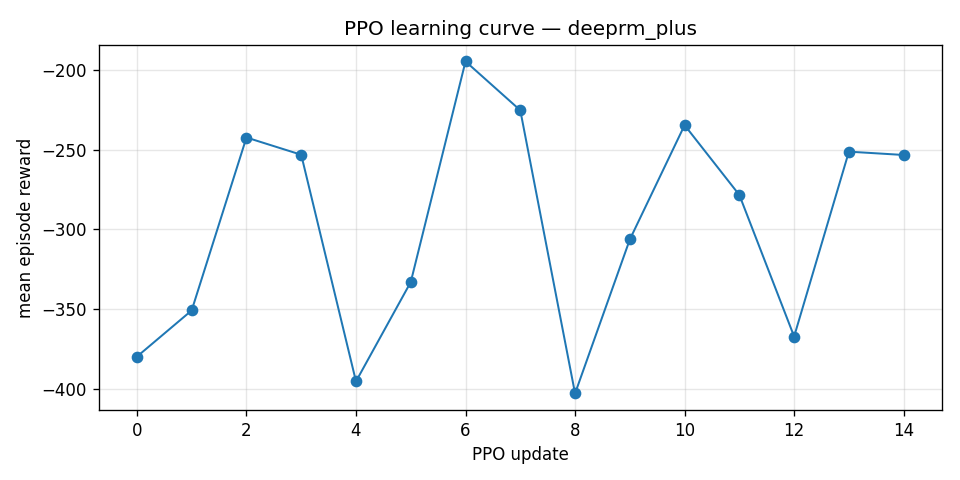
\includegraphics[width=\textwidth]{learning_curve_deeprm_plus.png}
\end{minipage}
\hfill
\begin{minipage}{0.49\textwidth}
\centering

\includegraphics[width=\textwidth]{learning_curve_deepreap.png}
\end{minipage}
\caption{PPO learning curves for DeepRM\_Plus (left) and DeepREAP
(right) over 15 updates. Both oscillate without converging; the
near-identical trajectories reflect the shared random seed. At this
budget, PPO refinement degrades both pre-trained policies.}
\label{fig:curves}
\end{figure}

We attribute this to budget rather than to a defect in the method. At
15 updates $\times$ 256 steps $\times$ 4 environments, PPO sees on the
order of $1.5 \times 10^4$ transitions --- far below the scale at which
policy-gradient methods stabilize on this class of problem. The
reward signal is also noisy: it aggregates over all resident jobs, so
a single long job entering the backlog perturbs it substantially.
Reporting these runs matters because the imitation checkpoint is the
result we would deploy, and readers should know it was reached by
supervised pre-training rather than by reinforcement learning.

\subsection{Operational Cost (RQ3)}

RQ3 asked about cost reduction for SMEs. We are not able to answer it.
Establishing a cost result requires a billing model, a real workload
and a deployment; our evaluation supplies none of these. The
completion-time reductions in Table~\ref{tab:bench} are consistent
with lower cost under a model that bills per unit of resource-time,
but the reduced throughput of the same policy pushes in the opposite
direction, and we have no basis for netting the two. We therefore
record RQ3 as open and note in Sect.~\ref{sec:future} what would be
needed to close it.

% =====================================================================
\subsection{Threats to Validity}

Our trace is parametric: although it reproduces diurnal cycles,
bimodal durations and dominant-resource demand, it is generated by a
process we also control, and a predictor may find it more forecastable
than a production trace would be --- the magnitude of the DeepREAP
gain should therefore be read as an upper bound. Results come from a
single trace at a single seed, so we report no confidence intervals
and make no significance claims. The 201-step budget truncates long
jobs and thus interacts with the very deferral behaviour that drives
DeepREAP's advantage; a longer horizon would let deferred jobs
complete and likely narrow the $n_{\text{done}}$ gap. Finally, the
scheduler runs in simulation, without network latency, failure
handling or multi-tenancy.

% =====================================================================
\section{Conclusion and Future Work}
\label{sec:future}
% =====================================================================

We set out to implement and evaluate DeepREAP, previously described
only as a conceptual architecture. The system now exists as working
software, and the integration hypothesis is supported on its primary
metric: injecting REAP demand forecasts into the scheduler's state
reduces average job slowdown by $2.4\times$ relative to the best
heuristic and by $2.3\times$ relative to an otherwise-identical
scheduler without forecasts. This answers RQ1 and, in part, RQ2.

The result is bounded in ways worth restating. The gain is
concentrated in the imitation-pretrained policy; our PPO refinement
stage degraded it. The gain comes with reduced throughput under a
fixed step budget. It is measured on a synthetic trace at a single
seed. And RQ3 --- operational cost for SMEs --- remains unanswered.

Priorities for future work follow directly. Scaling the RL budget by
an order of magnitude is the single most valuable next experiment, and
the environment, network and GAE pipeline already support it.
Substituting a real trace (Google cluster or Azure VM) is a
single-callsite change, since the generator already emits the
canonical schema. Softmax-with-temperature or top-$k$ ensemble
weighting should address the memory-target result in
Table~\ref{tab:reap-mem}; a reward combining slowdown with completion
count would let the policy trade latency against throughput
explicitly; re-fitting REAP online from live feedback would close the
loop the original architecture described; and pairing the simulator
with a provider billing model is the minimum needed to address RQ3.

\subsubsection{Reproducibility.}
All code, fixed seeds, trained checkpoints, raw benchmark output and
the scripts generating every figure are available in the project
repository.

% =====================================================================
\begin{thebibliography}{10}

\bibitem{guo2021}
Guo, W., Tian, W., Ye, Y., Xu, L., Wu, K.: Cloud resource scheduling
with deep reinforcement learning and imitation learning. IEEE Internet
of Things Journal \textbf{8}(5), 3576--3586 (2021).
\doi{10.1109/JIOT.2020.3025015}

\bibitem{savitha2021}
Savitha, S., Salvi, S.: Perceptive VM allocation in cloud data centers
for effective resource management. In: 6th International Conference
for Convergence in Technology (I2CT), pp. 1--5 (2021).
\doi{10.1109/I2CT51068.2021.9417960}

\bibitem{zhou2021}
Zhou, Z., Luo, K., Chen, X.: Deep reinforcement learning for
intelligent cloud resource management. In: IEEE INFOCOM Workshops,
pp. 1--6 (2021). \doi{10.1109/INFOCOMWKSHPS51825.2021.9484566}

\bibitem{mao2016}
Mao, H., Alizadeh, M., Menache, I., Kandula, S.: Resource management
with deep reinforcement learning. In: Proceedings of the 15th ACM
Workshop on Hot Topics in Networks, pp. 50--56 (2016).
\doi{10.1145/3005745.3005774}

\bibitem{osypanka2022}
Osypanka, P., Nawrocki, P.: Resource usage cost optimization in cloud
computing using machine learning. IEEE Transactions on Cloud Computing
\textbf{10}(3), 2079--2089 (2022). \doi{10.1109/TCC.2020.3015769}

\bibitem{osypanka2023}
Osypanka, P., Nawrocki, P.: QoS-aware cloud resource prediction for
computing services. IEEE Transactions on Services Computing
\textbf{16}(2), 1346--1357 (2023). \doi{10.1109/TSC.2022.3164256}

\bibitem{son2019}
Son, J., Buyya, R.: Priority-aware VM allocation and network bandwidth
provisioning in software-defined networking (SDN)-enabled clouds. IEEE
Transactions on Sustainable Computing \textbf{4}(1), 17--28 (2019).
\doi{10.1109/TSUSC.2018.2842074}

\bibitem{kaur2019}
Kaur, G., Bala, A., Chana, I.: An intelligent regressive ensemble
approach for predicting resource usage in cloud computing. Journal of
Parallel and Distributed Computing \textbf{123}, 1--12 (2019).
\doi{10.1016/j.jpdc.2018.08.008}

\bibitem{gyeera2023}
Gyeera, T.W., Simons, A.J.H., Stannett, M.: Regression analysis of
predictions and forecasts of cloud data center KPIs using the boosted
decision tree algorithm. IEEE Transactions on Big Data \textbf{9}(4),
1071--1085 (2023). \doi{10.1109/TBDATA.2022.3230649}

\bibitem{bankole2013}
Bankole, A.A., Ajila, S.A.: Predicting cloud resource provisioning
using machine learning techniques. In: 26th IEEE Canadian Conference
on Electrical and Computer Engineering (CCECE), pp. 1--4 (2013).
\doi{10.1109/CCECE.2013.6567848}

\end{thebibliography}

\end{document}
